\section{总体设计}
\subsection{概述}
本系统为基于大数据的舆情分析与预警系统,当今社会,互联网蓬勃发展,我们正处于一个一切皆有可能的大变革时代,纸媒、 微博、微信、APP正
在随时随地地影响着人们的生活,舆情场也随之改变,社会化媒体尤其是微博成为舆情爆发的主要阵地。本系统通过收集这些社会化媒体的数据,
对当前比较热门的话题等进行舆情分析,并对该舆情的发展方向进行预测,对可能出现的负面影响预警。

本系统设计为 B / S 架构,前端采用 HTML 5 + CSS 3 实现,后端采用 Spring + Spring MVC +Hadoop 框架实现,
本设计使系统具有优秀的解耦性,并大大增强了系统的可扩展性和可维护性。
\subsection{系统环境描述}
\subsubsection{运行环境}
\begin{itemize}
\item 软件环境
\end{itemize}

\begin{table}[!htbp]
	\centering
	\caption{软件环境}
	\label{tab:my-table}
	\begin{tabular}{|p{5cm}|p{4cm}|p{4cm}|}
		\hline
		分类 & 名称 & 版本 \\ \hline
		操作系统 & Linux(CentOS) & CentOS 7  \\ \hline
		数据库平台 & hadoop & 2.10.0  \\ \hline
		数据库平台 & MongoDB & 4.2  \\ \hline
		浏览器 & IE & IE9及以上  \\ \hline
	\end{tabular}
\end{table}
\newpage
\begin{itemize}
	\item 硬件环境
\end{itemize}	
\begin{table}[!htbp]
	\centering
	\caption{硬件环境}
	\label{tab:my-table1}
	\begin{tabular}{|p{5cm}|p{4cm}|p{4cm}|}
		\hline
		应用及服务器 & 最低配置 & 推荐配置 \\ \hline
		Mem & 8G & 32G \\ \hline
		HD & 160G & 600G \\ \hline
	\end{tabular}
\end{table}
\subsubsection{开发环境}
\begin{itemize}
	\item 开发机器软件环境
\end{itemize}
\begin{table}[!htbp]
	\centering
	\caption{开发机器软件环境}
	\label{tab:my-table2}
	\begin{tabular}{|p{5cm}|p{4cm}|p{4cm}|}
		\hline
		分类 & 名称 & 版本 \\ \hline
		操作系统 & Linux(CentOS) & CentOS 7  \\ \hline
		数据库平台 & hadoop & 2.10.0  \\ \hline
		数据库平台 & MongoDB & 4.2  \\ \hline
		浏览器 & IE & IE9及以上  \\ \hline
	\end{tabular}
\end{table}
\begin{itemize}
	\item 开发机器硬件环境
\end{itemize}	
\begin{table}[!htbp]
	\centering
	\caption{开发机器硬件环境}
	\label{tab:my-table3}
	\begin{tabular}{|p{5cm}|p{4cm}|p{4cm}|}
		\hline
		应用及服务器 & 最低配置 & 推荐配置 \\ \hline
		Mem & 8G & 32G \\ \hline
		HD & 160G & 600G \\ \hline
	\end{tabular}
\end{table}

\subsection{系统总体结构设计}

\subsubsection{系统业务层次图}
影视舆情分析系统是针对影视舆情数据进行分析,为个人用户提供实时的和可定制的舆情事件展示和分析,为企业用户(诸如电视台、影视剧投资方等)提供舆情事件预警和营销效果分析的系统,具有实时性、准确定、个性化等特点,系统共由8个模块组成:
\begin{figure}[!htbp]
	\centering
	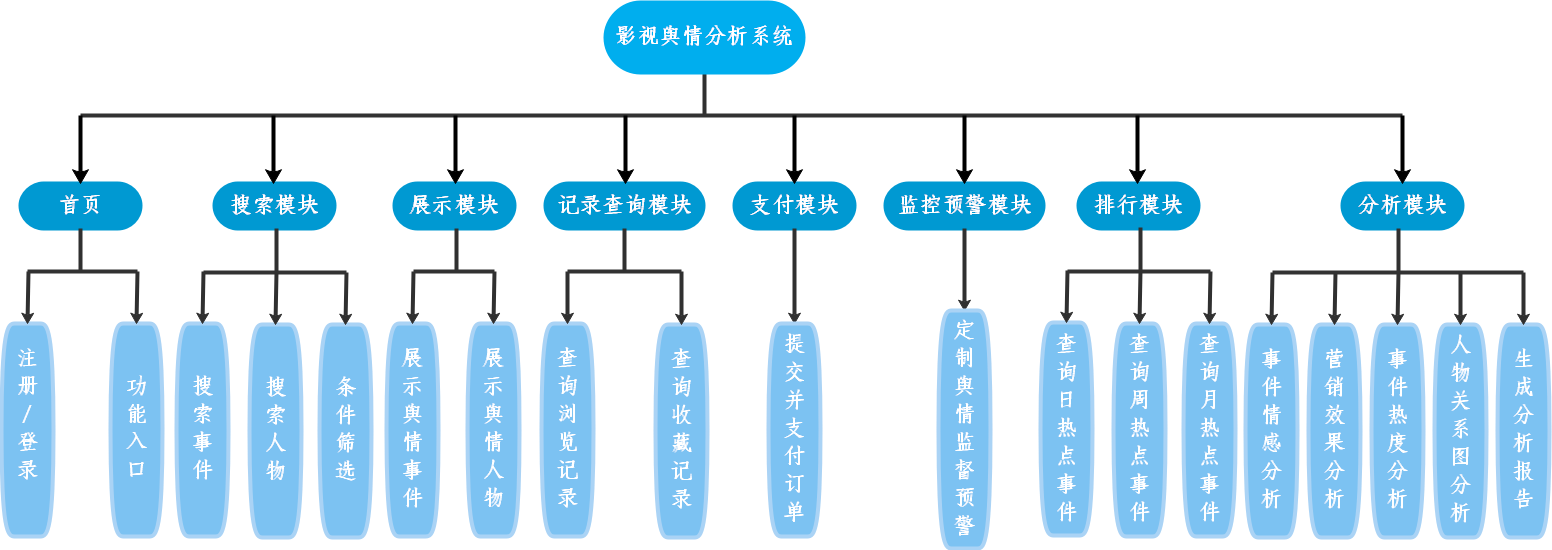
\includegraphics[scale=0.4]{image/o1.png}
	\caption{系统业务层次图}
\end{figure}


\subsubsection{模块功能介绍}

\begin{itemize}
	\item \textbf{首页}:提供用户注册、登录的功能按钮和个人/企业用户进入功能页面的模块;
	\item \textbf{搜索模块}:提供用户按照关键词搜索人物、时间的搜索功能或按一定条件(如职业、属地等)进行筛选的模块;
	\item \textbf{展示模块}:对事件发生的关键时间点,情感、热度变化和与人物有关的时间或关联人物可视化展示的模块;
	\item \textbf{记录查询模块}:提供对历史浏览记录和收藏查询的模块;
	\item \textbf{支付模块}:提供支付接口或查询支付记录的模块;
	\item \textbf{监控预警模块}:提供监控和预警定制和查看舆情预警的模块;
	\item \textbf{排行模块}:提供不同周期的热点事件排行榜的模块,具体时间周期为单日、本周和本月的热点事件排行榜;
	\item \textbf{分析模块}:提供影视舆情数据分析模块,可以对事件情感、热度和人物关系的分析进行查询,而企业用户可以对营销效果进行分析并生成分析报告。
	
\end{itemize}